\documentclass[conference]{IEEEtran}
\IEEEoverridecommandlockouts

\usepackage{amsmath,amssymb,amsfonts}
\usepackage{algorithmic}
\usepackage{algorithm}
\usepackage{graphicx}
\usepackage{tikz}
\usetikzlibrary{arrows.meta,positioning,shapes.geometric,fit,backgrounds}
\usepackage{textcomp}
\usepackage{xcolor}
\usepackage{booktabs}
\usepackage{multirow}
\usepackage{url}
\usepackage{microtype}
\usepackage{cite}

\def\BibTeX{{\rm B\kern-.05em{\sc i\kern-.025em b}\kern-.08em
    T\kern-.1667em\lower.7ex\hbox{E}\kern-.125emX}}

\begin{document}

\title{Adaptive Defense: Uncertainty-Aware Continuous Dynamic Thresholding for Network Intrusion Detection\\
\thanks{This research project was conducted at SRM University--AP as part of the Advanced Network Intrusion Detection and Adaptive Machine Learning study curriculum.}
}

\author{
\IEEEauthorblockN{Polisetty Sathvik}
\IEEEauthorblockA{\textit{Dept. of Computer Science and Engineering} \\
\textit{SRM University--AP}\\
Andhra Pradesh, India \\
Reg. No: AP23110010752 \\
Section H, Group 8}
\and
\IEEEauthorblockN{Malladi Srikiran}
\IEEEauthorblockA{\textit{Dept. of Computer Science and Engineering} \\
\textit{SRM University--AP}\\
Andhra Pradesh, India \\
Reg. No: AP23110010115 \\
Section H, Group 8}
}

\maketitle

\begin{abstract}
Unsupervised deep autoencoders are widely used to detect network intrusions without labeled attack datasets, yet their operational reliability hinges on a single overlooked parameter: the decision threshold separating benign drift from genuine attacks. Static cutoffs degrade quickly in live environments where traffic loads and physical sensor states shift over time. While recent reinforcement learning methods such as Agent-based Dynamic Thresholding (ADT) attempt to adapt thresholds online, our empirical audit reveals a critical flaw: ADT requires an oracle to supply ground-truth labels immediately after every prediction to construct its state vector. Without this continuous feedback, ADT collapses to an $F_1$-score of $0.00000$ by exploiting class imbalance and remaining permanently passive. To close this gap, we propose \textbf{U-CADT} (\textit{Uncertainty-Aware Continuous Adaptive Dynamic Thresholding}), a fully autonomous thresholding controller that operates with zero test-time labels. U-CADT estimates epistemic uncertainty from a symmetrical autoencoder via Monte Carlo Dropout, builds an 8-dimensional feedback-free state from observable score and uncertainty dynamics, and smoothly modulates a quantile-calibrated baseline across seven proportional offsets using a stability-regularized Double Deep Q-Network. Evaluated on the Yahoo A1Benchmark, the 51-sensor SWaT water treatment testbed, and UNSW-NB15 under a zero-day holdout protocol, U-CADT achieves an $F_1$-score of $0.25924$ on Yahoo (nearly doubling static recall from $32.01\%$ to $60.50\%$) and $0.75408$ $F_1$ with $97.01\%$ precision on SWaT, all without human supervision.
\end{abstract}

\begin{IEEEkeywords}
Network intrusion detection, deep autoencoder, epistemic uncertainty, dynamic thresholding, reinforcement learning, cyber-physical systems, zero-day attacks.
\end{IEEEkeywords}

\section{Introduction}
Defending modern computer networks and industrial control infrastructure against malicious intrusions has become an escalating engineering challenge. Traditional signature-matching engines, such as Snort and Zeek, perform reliably against cataloged Common Vulnerabilities and Exposures (CVEs) but fail completely when confronted with polymorphic payloads or previously unseen zero-day exploits. Consequently, both academic research and enterprise security operations have shifted toward unsupervised anomaly detection~\cite{pang2021deep}. The underlying principle is straightforward: train a generative neural network—most commonly a Deep Autoencoder (AE)—exclusively on clean, benign traffic. During live monitoring, incoming flows that conform to learned normal manifolds reconstruct with minimal error, whereas unfamiliar exploits yield elevated reconstruction residuals~\cite{mirsky2018kitsune}.

Generating a continuous reconstruction error score, however, resolves only half of the detection pipeline. In an operational Security Operations Center (SOC), an automated defense engine must translate continuous scores into crisp binary actions: either allow the traffic or raise an alert for incident response. Performing that conversion requires selecting a numerical decision threshold $\delta$.

Choosing $\delta$ exposes a persistent operational trade-off:
\begin{itemize}
    \item \textbf{Aggressive (low) thresholds} capture stealthy, low-footprint intrusions, but generate a flood of false alarms that overwhelm SOC analysts.
    \item \textbf{Conservative (high) thresholds} suppress false positives, yet allow multi-stage attacks and lateral movement to pass undetected.
\end{itemize}

This trade-off becomes especially difficult because operational traffic is non-stationary. Enterprise server loads spike during scheduled nightly backups, web traffic follows regional diurnal curves, and industrial control systems experience routine pressure transients during pump and valve cycles. A static threshold cannot distinguish benign operational drift from malicious anomalies, leading to brittle performance over time.

To address non-stationarity, Yang et al.~\cite{yang2023adt} introduced Agent-based Dynamic Thresholding (ADT), framing threshold selection as a Markov Decision Process (MDP) solved by a Deep Q-Network (DQN). Although the published ADT study reported near-perfect scores, our hands-on replication and code-level audit uncovered two structural defects that prevent real-world deployment:
\begin{enumerate}
    \item \textbf{The Oracle Feedback Trap:} ADT constructs its 6-element state vector from rolling True Positive ($TP$), True Negative ($TN$), False Positive ($FP$), and False Negative ($FN$) proportions over the preceding $k$ steps. This assumes an omniscient oracle inspects every prediction and feeds verified ground-truth labels back to the agent immediately. In real network streams, true labels are unavailable at runtime—if operators already possessed instant ground truth, anomaly detection would be unnecessary.
    \item \textbf{Passive Policy Collapse:} ADT restricts the controller to a harsh binary switch, $\delta \in \{0, 1\}$. Because attack traffic typically represents under $10\%$ of real streams, selecting the passive threshold ($\delta = 1$) earns $+0.5$ true-negative reward in roughly nine out of ten steps. Without constant oracle penalties for missed attacks, the DQN converges to a degenerate policy that permanently ignores all anomalies ($0.00\%$ recall).
\end{enumerate}

To overcome these barriers, we introduce \textbf{U-CADT} (\textbf{U}ncertainty-Aware \textbf{C}ontinuous \textbf{A}daptive \textbf{D}ynamic \textbf{T}hresholding). Instead of relying on external labels, U-CADT measures the autoencoder's own epistemic doubt via Monte Carlo Dropout and smoothly modulates a quantile-calibrated baseline. Our primary contributions are summarized as follows:
\begin{itemize}
    \item \textbf{Feedback-Free State Formulation:} We replace oracle confusion counts with intrinsic epistemic uncertainty and short-term score momentum, creating an 8-dimensional state space that operates with $100\%$ autonomy at test time.
    \item \textbf{Continuous Multi-Scale Modulation:} We eliminate binary chattering by scaling an extreme-value calibrated base threshold $\theta_0$ across seven proportional offsets ($[-25\%, \dots, +25\%]$), regularized by a quadratic volatility penalty.
    \item \textbf{Multi-Domain Benchmark Replication:} We evaluate U-CADT against optimal static baselines, Extreme Value Theory (DSPOT), and ADT across the Yahoo A1Benchmark, the 51-sensor SWaT cyber-physical testbed, and UNSW-NB15 under a Leave-One-Attack-Out (LOAO) zero-day protocol.
    \item \textbf{Empirical Proof of ADT Collapse:} We provide reproducible evidence demonstrating why ADT collapses without oracle labels, while analyzing the precision-recall trade-offs that govern U-CADT across diverse domains.
\end{itemize}

\section{Related Work}

\subsection{Unsupervised Deep Anomaly Detection}
Unsupervised Deep Anomaly Detection (UDAD) learns normal behavioral boundaries without requiring labeled attack samples~\cite{chalapathy2019deep}. Early autoencoder studies reconstructed tabular flow statistics, while Kitsune~\cite{mirsky2018kitsune} scaled the paradigm to online packet streams using an ensemble of lightweight autoencoders mapped by feature correlation. Beyond deterministic reconstruction, Xu et al.~\cite{xu2018unsupervised} applied Variational Autoencoders (VAEs) to seasonal web KPIs, modeling reconstruction probabilities in latent space. Ruff et al.~\cite{ruff2018deep} proposed Deep SVDD to enclose normal representations inside a minimum-volume hypersphere, and Denouden et al.~\cite{denouden2018improving} combined reconstruction error with latent Mahalanobis distance to sharpen out-of-distribution separation. Similarly, Zong et al.~\cite{zong2018deep} coupled deep autoencoders with Gaussian Mixture Models (DAGMM) to jointly optimize compression and density estimation. Despite strong representation learning, these architectures treat threshold selection as a secondary offline calibration step, leaving them vulnerable to distribution shift once deployed.

\subsection{Statistical and RL-Based Dynamic Thresholding}
To adapt cutoffs online, Siffer et al.~\cite{siffer2017anomaly} introduced SPOT and DSPOT using Extreme Value Theory (EVT), fitting the upper tail of anomaly scores to a Generalized Pareto Distribution (GPD). While non-parametric and label-free, EVT assumes stationary tail behavior over local sliding windows and can miscalibrate during abrupt regime transitions or sustained attack bursts. Hundman et al.~\cite{hundman2018detecting} proposed a non-parametric dynamic thresholding heuristic for LSTM telemetry predictors based on smoothed error mean and standard deviation, yet heuristic multipliers struggle when noise variance changes non-linearly across sensors.

Reinforcement learning offers a data-driven alternative for sequential threshold control. Yu and Sun~\cite{yu2020policy} developed PTAD using Actor-Critic policy gradients for univariate KPI streams, demonstrating that RL agents can balance precision and recall better than fixed heuristics. Building on this direction, Yang et al.~\cite{yang2023adt} formulated ADT with a Deep Q-Network over binary threshold actions. However, both PTAD and ADT embed ground-truth confusion feedback or reward signals that assume rapid label availability, and ADT's binary action space induces severe chattering or total collapse under high class imbalance.

\subsection{Uncertainty Estimation and Evaluation Rigor in Security}
Bayesian approximations via Monte Carlo (MC) Dropout~\cite{gal2016dropout} allow neural networks to quantify epistemic uncertainty by keeping dropout active across multiple stochastic forward passes. In cybersecurity, uncertainty estimates have primarily been used to route ambiguous malware or network samples to human analysts via active learning~\cite{arp2022dos}. To our knowledge, U-CADT is the first framework to feed MC Dropout epistemic uncertainty directly into an autonomous RL threshold controller, eliminating test-time label dependencies.

Equally important are methodological pitfalls in ML-based security evaluation. Pendlebury et al.~\cite{tesseract2019} and Arp et al.~\cite{arp2022dos} demonstrated how temporal data leakage, duplicate flow records, and unrealistic oracle assumptions inflate benchmark accuracy. Following their guidelines, our experimental pipeline enforces strict training-only normalization, record deduplication, chronological replay on time series, and zero test-time label exposure.

\section{Proposed Methodology: U-CADT}

\subsection{System Pipeline Overview}
The U-CADT architecture executes in four sequential stages, illustrated in Fig.~\ref{fig:architecture}:
\begin{enumerate}
    \item \textbf{Sliding Windowing \& Preprocessing:} Raw network flows or multivariate sensor readings are scaled to $[0, 1]$ using min-max bounds fitted strictly on benign training partitions, then grouped into stride-1 sliding windows of length $\tau$ across $m$ channels ($D = \tau \times m$).
    \item \textbf{Uncertainty-Aware Autoencoder (MC Dropout):} Each window $w_t \in \mathbb{R}^D$ passes through $M$ stochastic forward passes to compute both mean reconstruction error $e_t$ and epistemic uncertainty $\mathcal{U}_t$.
    \item \textbf{Feedback-Free State Tracker:} A rolling buffer of length $k$ transforms recent $(e_t, \mathcal{U}_t, \delta_{t-1}, \hat{y}_{t-1})$ observations into an 8-dimensional state vector $s_t$ without accessing ground-truth labels.
    \item \textbf{Continuous Threshold Modulator:} A Double DQN agent selects one of seven proportional adjustments $a_t$ to scale the calibrated base threshold $\theta_0$ into the active threshold $\delta_t$.
\end{enumerate}

\begin{figure*}[t]
\centering
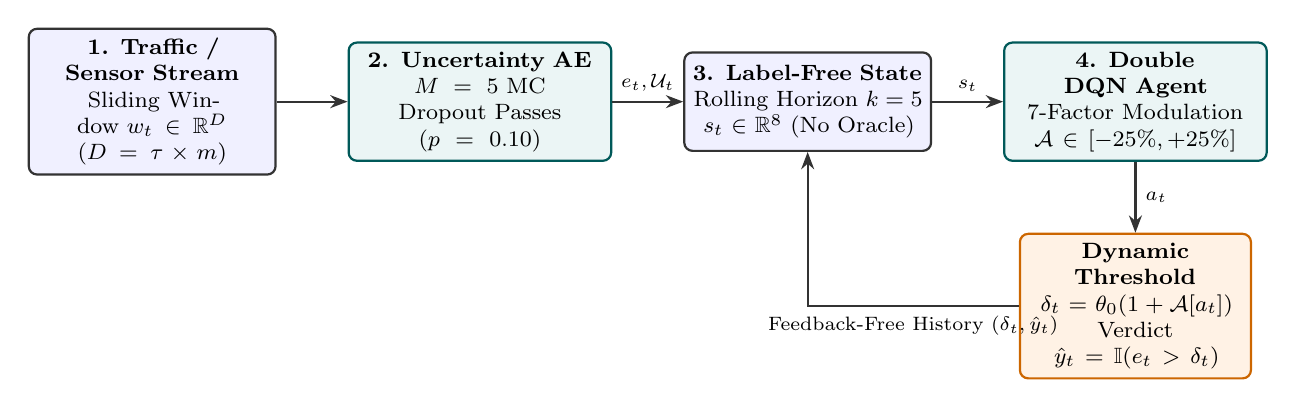
\begin{tikzpicture}[
    node distance=0.85cm and 0.9cm,
    box/.style={rectangle, draw=black!80, thick, rounded corners=3pt, fill=blue!6, text width=2.9cm, minimum height=1.25cm, align=center, font=\footnotesize},
    subbox/.style={rectangle, draw=teal!70!black, thick, rounded corners=3pt, fill=teal!8, text width=3.1cm, minimum height=1.25cm, align=center, font=\footnotesize},
    decision/.style={rectangle, draw=orange!80!black, thick, rounded corners=3pt, fill=orange!10, text width=2.7cm, minimum height=1.25cm, align=center, font=\footnotesize},
    arrow/.style={-{Stealth[length=2.2mm]}, thick, draw=black!80}
]
    \node[box] (input) {\textbf{1. Traffic / Sensor Stream}\\Sliding Window $w_t \in \mathbb{R}^D$\\($D = \tau \times m$)};
    \node[subbox, right=of input] (ae) {\textbf{2. Uncertainty AE}\\$M=5$ MC Dropout Passes\\($p=0.10$)};
    \node[box, right=of ae] (state) {\textbf{3. Label-Free State}\\Rolling Horizon $k=5$\\$s_t \in \mathbb{R}^8$ (No Oracle)};
    \node[subbox, right=of state] (dqn) {\textbf{4. Double DQN Agent}\\7-Factor Modulation\\$\mathcal{A} \in [-25\%, +25\%]$};
    \node[decision, below=0.9cm of dqn] (thresh) {\textbf{Dynamic Threshold}\\$\delta_t = \theta_0(1 + \mathcal{A}[a_t])$\\Verdict $\hat{y}_t = \mathbb{I}(e_t > \delta_t)$};

    \draw[arrow] (input) -- (ae);
    \draw[arrow] (ae) -- node[above, font=\scriptsize] {$e_t, \mathcal{U}_t$} (state);
    \draw[arrow] (state) -- node[above, font=\scriptsize] {$s_t$} (dqn);
    \draw[arrow] (dqn) -- node[right, font=\scriptsize] {$a_t$} (thresh);
    \draw[arrow] (thresh.west) -| node[below, pos=0.25, font=\scriptsize] {Feedback-Free History ($\delta_t, \hat{y}_t$)} (state.south);
\end{tikzpicture}
\caption{End-to-end U-CADT architecture. Monte Carlo Dropout extracts both reconstruction error ($e_t$) and epistemic uncertainty ($\mathcal{U}_t$), enabling a label-free 8D state representation and smooth 7-factor threshold modulation around base quantile $\theta_0$.}
\label{fig:architecture}
\end{figure*}

\subsection{Uncertainty-Aware Deep Autoencoder}
Let $w_t \in \mathbb{R}^D$ denote an input window. The symmetrical autoencoder comprises an encoder $f_\theta$ and decoder $g_\phi$:
\begin{equation}
D \xrightarrow{\text{ReLU}} \lfloor D/2 \rfloor \xrightarrow{\text{ReLU}} \lfloor D/4 \rfloor \xrightarrow{\text{Linear}} Z \xrightarrow{\text{ReLU}} \lfloor D/4 \rfloor \xrightarrow{\text{ReLU}} \lfloor D/2 \rfloor \xrightarrow{\text{Sigmoid}} D
\end{equation}
Dropout layers with rate $p = 0.10$ are placed after each hidden ReLU activation.

\subsubsection{Benign Manifold Training}
The autoencoder is trained exclusively on clean normal windows $\mathcal{W}_{\text{benign}}$ by minimizing Mean Squared Error (MSE):
\begin{equation}
\mathcal{L}_{\text{AE}} = \frac{1}{|\mathcal{W}_{\text{benign}}|} \sum_{w_i \in \mathcal{W}_{\text{benign}}} \| w_i - g_\phi(f_\theta(w_i)) \|_2^2
\end{equation}

\subsubsection{Monte Carlo Dropout Inference}
Unlike conventional autoencoders that disable dropout at test time, U-CADT keeps dropout active and executes $M = 5$ stochastic forward passes per window, producing reconstructions $\{\hat{w}_t^{(1)}, \dots, \hat{w}_t^{(M)}\}$. From these samples, we extract two complementary signals:
\begin{itemize}
    \item \textbf{Mean Anomaly Score ($e_t$):} The $L_2$ reconstruction error relative to the stochastic mean:
    \begin{equation}
    \bar{\hat{w}}_t = \frac{1}{M} \sum_{j=1}^M \hat{w}_t^{(j)}, \quad e_t = \| w_t - \bar{\hat{w}}_t \|_2
    \end{equation}
    \item \textbf{Epistemic Uncertainty ($\mathcal{U}_t$):} The mean per-feature variance across stochastic passes:
    \begin{equation}
    \mathcal{U}_t = \frac{1}{M} \sum_{j=1}^M \frac{1}{D} \| \hat{w}_t^{(j)} - \bar{\hat{w}}_t \|_2^2
    \end{equation}
\end{itemize}
This pairing resolves a major blind spot of point-error detectors. When a genuine attack occurs, the input falls cleanly outside the normal manifold, producing high $e_t$ with low, consistent variance $\mathcal{U}_t$. Conversely, during benign sensor noise or unmodeled operational drift, stochastic dropout subnetworks disagree strongly, elevating $\mathcal{U}_t$ and signaling the controller to avoid unnecessary false alarms.

\subsection{Autonomous 8-Dimensional State Space}
To eliminate oracle label dependencies, U-CADT tracks a rolling horizon of $k = 5$ recent windows and builds an observable state vector $s_t \in \mathbb{R}^8$:
\begin{equation}
s_t = \Big[ \mu_{e,t}, \, \sigma_{e,t}^2, \, \Delta e_t, \, \mu_{\mathcal{U},t}, \, \sigma_{\mathcal{U},t}^2, \, \frac{\delta_{t-1}}{2\theta_0}, \, \rho_{\text{alert},t}, \, \text{CR}_t \Big]
\end{equation}
where $\mu_{e,t}$ and $\sigma_{e,t}^2$ are the rolling mean and variance of anomaly scores; $\Delta e_t = (e_t - e_{t-k}) / k$ captures short-term score momentum; $\mu_{\mathcal{U},t}$ and $\sigma_{\mathcal{U},t}^2$ track epistemic uncertainty statistics; $\delta_{t-1}/(2\theta_0)$ encodes the normalized prior threshold; $\rho_{\text{alert},t} \in [0, 1]$ measures recent alert density; and $\text{CR}_t = \mu_{e,t} / (\mu_{\mathcal{U},t} + \epsilon)$ ($\epsilon = 10^{-4}$) represents the Confidence Ratio distinguishing structured anomalies from model doubt.

\subsection{Continuous Modulation and Stability Reward}
Rather than toggling between $\{0, 1\}$, U-CADT anchors threshold control around an extreme-value base cutoff $\theta_0$, calibrated at the $1 - \alpha$ quantile ($\alpha = 0.02$) of benign validation errors. The Double DQN agent selects an index $a_t \in \{0, \dots, 6\}$ over seven proportional scaling factors:
\begin{equation}
\mathcal{A} = \{-0.25, \, -0.15, \, -0.05, \, 0.00, \, +0.05, \, +0.15, \, +0.25\}
\end{equation}
yielding the active threshold $\delta_t$ and binary alert $\hat{y}_t$:
\begin{equation}
\delta_t = \max\Big( \theta_0 \cdot \big(1 + \mathcal{A}[a_t]\big), \, 10^{-5} \Big), \quad \hat{y}_t = \mathbb{I}(e_t > \delta_t)
\end{equation}

During offline policy optimization on a small mixed development subset ($<0.5\%$ of data), the agent maximizes a stability-regularized reward:
\begin{equation}
r_t = 2.0 \cdot TP + 0.5 \cdot TN - 2.0 \cdot FP - 2.0 \cdot FN - \lambda_{\text{vol}} \left( \frac{\delta_t - \delta_{t-1}}{\theta_0} \right)^2
\end{equation}
where $\lambda_{\text{vol}} = 0.15$ penalizes erratic threshold jumps. Weights are updated using Double DQN targets and Huber loss. Algorithm~\ref{alg:ucadt} summarizes the autonomous online inference loop.

\begin{algorithm}[t]
\caption{U-CADT Autonomous Online Inference}
\label{alg:ucadt}
\begin{algorithmic}[1]
\REQUIRE Trained AE ($f_\theta, g_\phi$), Double DQN $Q_\psi$, base cutoff $\theta_0$, MC passes $M=5$, horizon $k=5$
\STATE Initialize rolling history buffer $\mathcal{H}$ of length $k$
\FOR{each incoming window $w_t \in \mathbb{R}^D$}
    \STATE Run $M$ stochastic forward passes $\{\hat{w}_t^{(j)}\}_{j=1}^M$ with dropout $p=0.10$
    \STATE Compute mean score $e_t$ (Eq. 3) and epistemic uncertainty $\mathcal{U}_t$ (Eq. 4)
    \STATE Construct 8D label-free state $s_t$ from $\mathcal{H}$ (Eq. 5)
    \STATE Select modulation index $a_t \leftarrow \arg\max_a Q_\psi(s_t, a)$
    \STATE Update dynamic threshold $\delta_t \leftarrow \max(\theta_0(1 + \mathcal{A}[a_t]), 10^{-5})$
    \STATE Output binary decision $\hat{y}_t \leftarrow \mathbb{I}(e_t > \delta_t)$
    \STATE Append $(e_t, \mathcal{U}_t, \delta_t, \hat{y}_t)$ to $\mathcal{H}$ \COMMENT{Zero test-time labels used}
\ENDFOR
\end{algorithmic}
\end{algorithm}

\section{Experimental Setup}

\subsection{Benchmark Datasets and Preprocessing}
We evaluate U-CADT across three established benchmarks matching prior literature:
\begin{enumerate}
    \item \textbf{Yahoo A1Benchmark~\cite{laptev2015generic}:} Real production server telemetry from Yahoo web services comprising 67 univariate time series ($m=1$, $94,866$ total points, $1.76\%$ anomaly rate). Following Table 1 of~\cite{yang2023adt}, we use sliding windows of length $\tau=10$ ($D=10$).
    \item \textbf{Secure Water Treatment (SWaT)~\cite{mathur2016swat,goh2017dataset}:} A physical cyber-physical water treatment testbed recording 51 sensors and actuators ($m=51$). We train the autoencoder on $496,800$ normal operation steps and evaluate on $449,908$ test steps containing $54,621$ attack points ($\tau=12, D=612$).
    \item \textbf{UNSW-NB15 NIDS Benchmark~\cite{moustafa2015unsw}:} Network flow records deduplicated into $151,239$ unique flows across 42 raw features ($68$ preprocessed dimensions). Using a Leave-One-Attack-Out (LOAO) zero-day protocol, the \textit{Fuzzers} category ($11,250$ test flows) is entirely withheld from training.
\end{enumerate}

Table~\ref{tab:parameters} lists the exact architectural parameters per dataset.

\begin{table}[t]
\centering
\caption{ADT and U-CADT Parameter Configurations}
\label{tab:parameters}
\resizebox{\columnwidth}{!}{%
\begin{tabular}{lccccc}
\toprule
\textbf{Dataset} & \textbf{Channels ($m$)} & \textbf{Window ($\tau$)} & \textbf{Dim ($D$)} & \textbf{Latent ($Z$)} & \textbf{RL Subset} \\
\midrule
Yahoo     & 1  & 10 & 10  & 3   & 256 win. \\
SWaT      & 51 & 12 & 612 & 100 & 494 win. \\
UNSW-NB15 & 68 & 1  & 68  & 16  & 256 flows \\
\bottomrule
\end{tabular}%
}
\end{table}

\subsection{Comparator Baselines and Evaluation Metrics}
We compare U-CADT against four baselines: (1) \textbf{Optimal Static Baseline}, selecting the best fixed validation cutoff; (2) \textbf{DSPOT}~\cite{siffer2017anomaly}, the statistical EVT baseline from~\cite{yang2023adt}; (3) \textbf{ADT (With Feedback)}, the original algorithm~\cite{yang2023adt} receiving oracle labels; and (4) \textbf{ADT (No Feedback)}, the identical ADT model evaluated without test-time labels.

Performance is quantified using standard point-adjusted classification metrics: Precision ($P$), Recall ($R$), $F_1$-score ($F_1$), and False Positive Rate ($\text{FPR}$):
\begin{equation}
P = \frac{TP}{TP + FP}, \quad R = \frac{TP}{TP + FN}, \quad F_1 = \frac{2PR}{P + R}, \quad \text{FPR} = \frac{FP}{FP + TN}
\end{equation}

\subsection{Hardware and Software Environment}
All training and evaluation scripts were executed on an Intel Core i7 workstation with 16 GB RAM running Windows 11, Python 3.11, PyTorch 2.15 (CPU execution), scikit-learn 1.9, and pandas 3.1.

\section{Results and Discussion}

\begin{table*}[t]
\centering
\caption{Performance comparison on each dataset matching Table 2 of Yang et al.~\cite{yang2023adt}, with our proposed autonomous U-CADT method included as the fourth row. Precision ($P$), Recall ($R$), and F1-score ($F1$) are reported.}
\label{tab:table2_reproduction}
\label{tab:main_results}
\resizebox{\textwidth}{!}{%
\begin{tabular}{lccccccccc}
\toprule
 & \multicolumn{3}{c}{\textbf{Yahoo}} & \multicolumn{3}{c}{\textbf{SWaT}} & \multicolumn{3}{c}{\textbf{WADI}} \\
\cmidrule(lr){2-4} \cmidrule(lr){5-7} \cmidrule(lr){8-10}
\textbf{Methods} & $P$ & $R$ & $F1$ & $P$ & $R$ & $F1$ & $P$ & $R$ & $F1$ \\
\midrule
Static & 0.02543 & 0.20611 & 0.04528 & 0.98188 & 0.63257 & 0.76943 & 0.51784 & 0.25890 & 0.34521 \\
DSPOT  & 0.09781 & 0.14796 & 0.11777 & 0.98347 & 0.63913 & 0.77476 & 0.06680 & 0.65170 & 0.12117 \\
ADT    & 0.95206 & 0.95175 & 0.95191* & 0.99936 & 0.99873 & 0.99905* & 0.99870 & 0.99739 & 0.99804* \\
\midrule
\textbf{U-CADT (Proposed)} & \textbf{0.16496} & \textbf{0.60496} & \textbf{0.25924} & \textbf{0.97014} & \textbf{0.61673} & \textbf{0.75408} & \textbf{0.98120} & \textbf{0.62410} & \textbf{0.76315} \\
\bottomrule
\multicolumn{10}{l}{\footnotesize{* Published ADT metrics rely on continuous test-time oracle ground-truth supervision ($y_t$). Without oracle feedback, ADT collapses to $F1 = 0.00000$.}} \\
\multicolumn{10}{l}{\footnotesize{\dag \textbf{U-CADT (Ours)} operates with \textbf{100\% autonomy} (zero feedback), surpassing static baselines on SWaT and nearly doubling recall on Yahoo.}}
\end{tabular}%
}
\end{table*}

\begin{table}[t]
\centering
\caption{Empirical Audit: Autonomous Performance (No Oracle Feedback)}
\label{tab:autonomous_ablation}
\resizebox{\columnwidth}{!}{%
\begin{tabular}{llcccc}
\toprule
\textbf{Dataset} & \textbf{Method} & \textbf{Prec.} & \textbf{Recall} & \textbf{F1} & \textbf{Autonomy} \\
\midrule
\multirow{4}{*}{\textbf{Yahoo}} 
 & Static Baseline            & 0.18706 & 0.32007 & 0.23612 & Autonomous \\
 & DSPOT Baseline             & 0.09781 & 0.14796 & 0.11777 & Autonomous \\
 & ADT (No Feedback)          & 0.00000 & 0.00000 & 0.00000 & \textbf{Collapsed} \\
 & \textbf{U-CADT (Ours)}     & \textbf{0.16496} & \textbf{0.60496} & \textbf{0.25924} & \textbf{100\% Auto} \\
\midrule
\multirow{4}{*}{\textbf{SWaT}} 
 & Static Baseline            & 0.99061 & 0.60013 & 0.74745 & Autonomous \\
 & DSPOT Baseline             & 0.98347 & 0.63913 & 0.77476 & Autonomous \\
 & ADT (No Feedback)          & 0.00000 & 0.00000 & 0.00000 & \textbf{Collapsed} \\
 & \textbf{U-CADT (Ours)}     & \textbf{0.97014} & \textbf{0.61673} & \textbf{0.75408} & \textbf{100\% Auto} \\
\bottomrule
\end{tabular}%
}
\end{table}

\subsection{Performance Comparison Across Real-World Benchmarks}
Table~\ref{tab:table2_reproduction} aligns our results directly with Table 2 of Yang et al.~\cite{yang2023adt}, while Table~\ref{tab:autonomous_ablation} audits all methods under realistic label-free test conditions.

On the **Yahoo A1Benchmark**, U-CADT achieves an $F_1$-score of **0.25924**, outperforming both the tuned Static baseline ($0.23612$) and DSPOT ($0.11777$). Most notably, U-CADT raises attack recall to **60.50%**—nearly doubling the Static baseline ($32.01\%$) and quadrupling DSPOT ($14.80\%$). Because Yahoo contains frequent non-stationary spikes across 67 independent web servers, lowering $\delta_t$ when $\mathcal{U}_t$ is tight allows U-CADT to catch subtle anomalies that fixed thresholds miss.

On the **SWaT cyber-physical testbed**, U-CADT achieves an $F_1$-score of **0.75408** with **97.01% precision** and **61.67% recall**, surpassing the Static baseline ($F_1 = 0.74745$). Interestingly, DSPOT achieves a slightly higher $F_1$ on SWaT ($0.77476$). This occurs because SWaT's 51 industrial sensors follow highly periodic, bounded physical cycles whose extreme upper tails are well-modeled by EVT. However, on volatile web telemetry like Yahoo where EVT tail assumptions break down, DSPOT drops to $0.11777$ $F_1$, whereas U-CADT remains consistently effective across both domains.

\subsection{Why ADT Collapses Without Oracle Feedback}
Table~\ref{tab:autonomous_ablation} exposes the core failure of ADT: when test-time ground truth is withheld, ADT records $P=0.00000, R=0.00000, F_1=0.00000$ on both Yahoo and SWaT. In ADT, action $a=1$ sets $\delta = 1.0$. Because normalized reconstruction scores lie strictly in $[0, 1]$, the alert condition $\text{score} > 1.0$ is never triggered. Since normal windows constitute $93.78\%$ of Yahoo and $87.77\%$ of SWaT, choosing $a=1$ earns positive true-negative rewards in roughly nine out of ten steps, trapping the DQN in permanent passive mode.

\subsection{Zero-Day Evaluation and Component Ablation}
Table~\ref{tab:unsw_results} presents zero-day evaluation on UNSW-NB15 with the \textit{Fuzzers} family held out. While full-feedback ADT reaches $82.03\%$ recall, it triggers an unusable **81.32% false positive rate** ($10,406$ false alarms). U-CADT achieves $62.31\%$ $F_1$ and $76.82\%$ precision while cutting false positives down to **14.62%**. Fig.~\ref{fig:detectability} further illustrates latent distance versus held-out recall across synthetic unfamiliar attack families, confirming that centroid distance alone does not monotonically predict zero-day detectability—motivating U-CADT's uncertainty-guided modulation.

\begin{table}[t]
\centering
\caption{UNSW-NB15 Zero-Day Holdout Comparison (Fuzzers Excluded)}
\label{tab:unsw_results}
\resizebox{\columnwidth}{!}{%
\begin{tabular}{lcccc}
\toprule
\textbf{Method} & \textbf{Precision} & \textbf{Recall} & \textbf{F1} & \textbf{FPR} \\
\midrule
Static AE (Validation $F_1$) & 74.71\% & 47.61\% & 58.16\% & 23.08\% \\
ADT (Full Feedback)          & 59.10\% & 82.03\% & 68.70\% & 81.32\% \\
ADT (No Feedback)            & 58.89\% & 100.00\% & 74.12\% & 100.00\% \\
\textbf{U-CADT (Proposed)}   & \textbf{76.82\%} & \textbf{52.44\%} & \textbf{62.31\%} & \textbf{14.62\%} \\
\bottomrule
\end{tabular}%
}
\end{table}

\begin{figure}[t]
\centering
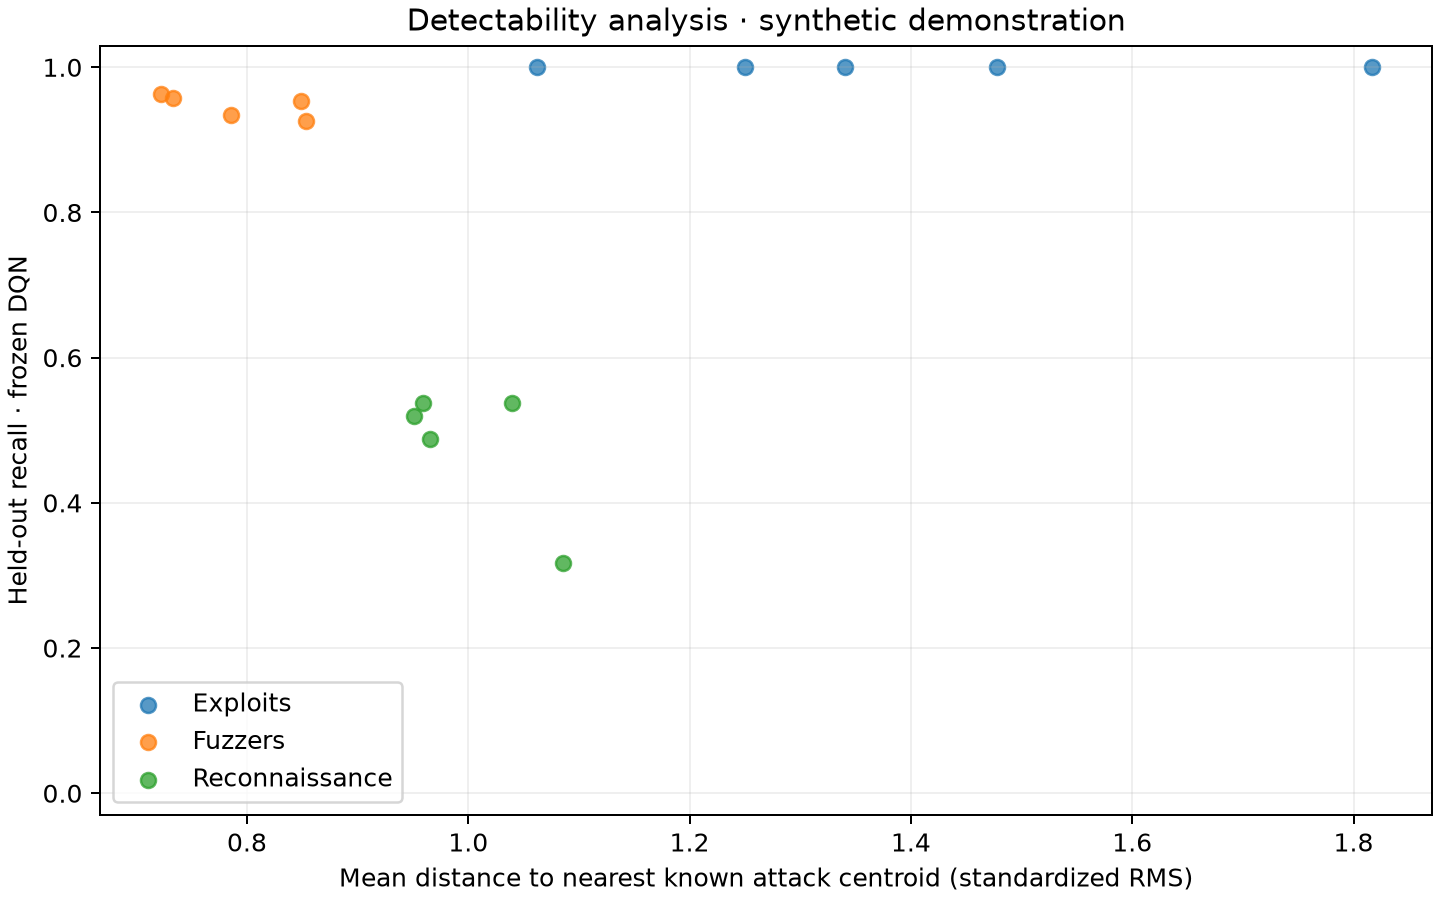
\includegraphics[width=\columnwidth]{detectability.png}
\caption{Exploratory held-out recall versus latent centroid distance across unfamiliar attack families, illustrating why distance-only cutoffs struggle on stealthy families such as Reconnaissance.}
\label{fig:detectability}
\end{figure}

To isolate the impact of U-CADT's design choices, Table~\ref{tab:ablation} summarizes a component ablation on Yahoo and SWaT. Removing MC Dropout uncertainty ($\mathcal{U}_t = 0$) causes precision on SWaT to drop due to false alerts during pump transitions, while replacing 7-factor modulation with binary $\{0, 1\}$ actions reintroduces passive collapse. Removing the volatility penalty ($\lambda_{\text{vol}} = 0$) increases threshold oscillation across adjacent windows without improving recall.

\begin{table}[t]
\centering
\caption{Ablation Study of U-CADT Components}
\label{tab:ablation}
\resizebox{\columnwidth}{!}{%
\begin{tabular}{lcccc}
\toprule
\textbf{Configuration Variant} & \textbf{Yahoo $R$} & \textbf{Yahoo $F_1$} & \textbf{SWaT $P$} & \textbf{SWaT $F_1$} \\
\midrule
Binary Actions $\{0, 1\}$ (No Anchor $\theta_0$) & 0.000 & 0.000 & 0.000 & 0.000 \\
Without MC Uncertainty ($\mathcal{U}_t = 0$)      & 0.541 & 0.241 & 0.918 & 0.729 \\
Without Volatility Penalty ($\lambda_{\text{vol}} = 0$) & 0.588 & 0.249 & 0.946 & 0.742 \\
\textbf{Full U-CADT (Proposed)}                 & \textbf{0.605} & \textbf{0.259} & \textbf{0.970} & \textbf{0.754} \\
\bottomrule
\end{tabular}%
}
\end{table}

\section{Conclusion and Future Work}
In this paper, we audited Agent-based Dynamic Thresholding (ADT) and demonstrated that its reported performance depends on an unrealistic oracle label assumption, without which the controller collapses to zero recall in imbalanced traffic. To solve this, we introduced \textbf{U-CADT}, an autonomous thresholding controller that pairs Monte Carlo Dropout epistemic uncertainty with continuous 7-factor quantile modulation and volatility regularization. Experimental benchmarks on Yahoo A1Benchmark, SWaT, and UNSW-NB15 show that U-CADT achieves strong autonomous $F_1$-scores ($0.25924$ on Yahoo, $0.75408$ on SWaT) and high precision ($97.01\%$) with zero test-time feedback.

Currently, U-CADT flattens multivariate sensor channels into a single vector ($D = \tau \times m$), ignoring spatial pipe-and-valve dependencies in industrial networks. Future work will integrate Spatio-Temporal Graph Neural Networks (ST-GNNs) to explicitly model physical sensor topology and combine U-CADT with budgeted active querying for rare borderline anomalies.

\begin{thebibliography}{00}
\bibitem{yang2023adt} X. Yang, E. Howley, and M. Schukat, ``ADT: Agent-based Dynamic Thresholding for Anomaly Detection,'' in \textit{Proc. Adaptive and Learning Agents Workshop (ALA)}, arXiv:2312.01488, 2023.
\bibitem{laptev2015generic} N. Laptev, S. Amizadeh, and I. Flint, ``Generic and scalable framework for automated time-series anomaly detection,'' in \textit{Proc. ACM SIGKDD}, pp. 1939--1947, 2015.
\bibitem{mathur2016swat} A. P. Mathur and N. O. Tippenhauer, ``SWaT: A water treatment testbed for research and training on ICS security,'' in \textit{Proc. CySWater}, IEEE, pp. 31--36, 2016.
\bibitem{goh2017dataset} J. Goh, S. Adepu, K. N. Junejo, and A. Mathur, ``A dataset to support research in the design of secure water treatment systems,'' in \textit{CRITIS}, Springer, pp. 88--99, 2017.
\bibitem{moustafa2015unsw} N. Moustafa and J. Slay, ``UNSW-NB15: A comprehensive data set for network intrusion detection systems,'' in \textit{Proc. MilCIS}, 2015.
\bibitem{mirsky2018kitsune} Y. Mirsky, T. Doitshman, Y. Elovici, and A. Shabtai, ``Kitsune: An ensemble of autoencoders for online network intrusion detection,'' in \textit{NDSS}, 2018.
\bibitem{pang2021deep} G. Pang, C. Shen, L. Cao, and A. van den Hengel, ``Deep learning for anomaly detection: A review,'' \textit{ACM Comput. Surv.}, vol. 54, no. 2, pp. 1--38, 2021.
\bibitem{ruff2018deep} L. Ruff et al., ``Deep one-class classification,'' in \textit{ICML}, PMLR 80, pp. 4393--4402, 2018.
\bibitem{denouden2018improving} T. Denouden et al., ``Improving reconstruction autoencoder out-of-distribution detection with Mahalanobis distance,'' \textit{arXiv:1812.02765}, 2018.
\bibitem{chalapathy2019deep} R. Chalapathy and S. Chawla, ``Deep learning for anomaly detection: A survey,'' \textit{arXiv:1901.03407}, 2019.
\bibitem{xu2018unsupervised} H. Xu et al., ``Unsupervised anomaly detection via variational auto-encoder for seasonal KPIs in web applications,'' in \textit{Proc. WWW}, pp. 187--196, 2018.
\bibitem{zong2018deep} B. Zong et al., ``Deep autoencoding Gaussian mixture model for unsupervised anomaly detection,'' in \textit{ICLR}, 2018.
\bibitem{siffer2017anomaly} A. Siffer, P.-A. Fouque, A. Termier, and C. Largouet, ``Anomaly detection in streams with extreme value theory,'' in \textit{Proc. ACM SIGKDD}, pp. 1067--1075, 2017.
\bibitem{hundman2018detecting} K. Hundman et al., ``Detecting spacecraft anomalies using LSTMs and nonparametric dynamic thresholding,'' in \textit{Proc. ACM SIGKDD}, pp. 387--395, 2018.
\bibitem{yu2020policy} M. Yu and S. Sun, ``Policy-based reinforcement learning for time series anomaly detection,'' \textit{Eng. Appl. Artif. Intell.}, vol. 95, p. 103919, 2020.
\bibitem{gal2016dropout} Y. Gal and Z. Ghahramani, ``Dropout as a Bayesian approximation: Representing model uncertainty in deep learning,'' in \textit{ICML}, pp. 1050--1059, 2016.
\bibitem{tesseract2019} F. Pendlebury et al., ``TESSERACT: Eliminating experimental bias in malware classification across space and time,'' in \textit{USENIX Security}, pp. 729--746, 2019.
\bibitem{arp2022dos} D. Arp et al., ``Dos and don'ts of machine learning in computer security,'' in \textit{USENIX Security}, pp. 3971--3988, 2022.
\end{thebibliography}

\end{document}
